\documentclass[article,
12pt, 
a4paper,  
%twoside,
english]{article}
\usepackage[english]{babel}
\usepackage{titling}
\linespread{1.05}
\usepackage{times} 
\usepackage[hmarginratio=1:1,top=25mm,left=20mm, columnsep=20pt]{geometry} 
\usepackage[hang, small,labelfont=bf,up,textfont=it,up]{caption} 
\usepackage{booktabs}
\usepackage{indentfirst}
\usepackage{enumitem}
\setlist[itemize]{noitemsep}
\usepackage{fancyhdr} % Headers and footers
\usepackage{titling} % Customizing the title section
\usepackage{hyperref} % For hyperlinks in the PDF
\usepackage{array} %permite o uso de tabelas
\usepackage{longtable} %permite o uso de tabelas personalizadas
\usepackage{rotating} %permite rotacionar imagens
\graphicspath{{./images/} }
\usepackage{subfiles} % Best loaded last in the preamble
\usepackage[language=english]{biblatex}
\addbibresource{references.bib} %Imports bibliography file
\usepackage{csquotes}
\usepackage[font={footnotesize}, labelfont=normalfont, textfont=up,]{caption}
\usepackage{setspace}

\captionsetup[figure]{labelfont={bf},name={Fig.},labelsep=period}
\captionsetup[table]{labelfont={bf},name={Table},labelsep=period}


\usepackage{abstract} % Allows abstract customization
\usepackage{titlesec} % Allows customization of titles
\titleformat{\section}[block]{\large\centering}{\thesection}{1em}{\MakeUppercase}{} % Change the look of the section titles
\titleformat{\subsection}[block]{\large}{\thesubsection.}{1em}{} % Change the look of the section titles
\nocite{*}

\renewcommand\maketitlehooka{\null\mbox{}\vfill}
\renewcommand\maketitlehookd{\vfill\null}

\title{Performance comparison between CPU and GPU based ray tracer} % Article title
\author{%
\textsc{Przemysław Kowalewski}
\normalsize \\ \href{mailto:pkow@kth.se}{pkow@kth.se} \\
\normalsize Code: \href{https://github.com/irqize/CudaRayTracer}{github.com/irqize/CudaRayTracer} \\
\normalsize Expected grade: A
}
\date{2022-01-02}

\begin{document}
\begin{titlingpage}
\maketitle
\end{titlingpage}
\onehalfspacing
\section{Introduction}

The aim of this report is to present the experiment carried out to compare the performances of the same naive ray tracing algorithm implemented in C++ one using only CPU and the second one performing most of the calculation on the GPU using the CUDA platform and uses CPU for the GPU memory allocation and copying the pixel data back from the GPU, kernel initialization and saving the image to file.

\section{Methodology}

The algorithm used to generate each pixel’s value is the same as in the Python code provided in paragraph B of the assignment. Firstly for the easy access of data I defined five C++ structs which are representations of a pixel, a material, a sphere a light, and a camera, after that I defined four helper functions responsible for calculating the dot product of two vectors, calculating a distance of a point of intersection of the ray from the camera with a sphere from the camera, creating a new normalized vector and clamping a value between 1 and 0. After that, there come two most important functions of the application 

The main function allocates required memory, defines required data structures, launches the kernel, and then saves the generated image using the EasyBMP library. The GPU version additionally also transfers the data to and from the GPU. 

The kernel is responsible for rendering singular pixel, firstly it checks if the ray from this pixel’s position intersects the sphere if it doesn’t it sets the pixel to black. Otherwise, the algorithm continues and calculates the color with the Blinn-Phong shading model with ambient, diffuse, and specular lighting components, it adds these components up to one color and saves it in the image representation

To compare the implementations I chose the optimal block size configuration for the GPU version by running it three times and measuring the time of execution and choosing the one with the smallest average. After that, for each version and resolution, I ran the algorithms, measured the average time of execution and standard deviation of these measurements and the time required to render one pixel.

\section{Experimental setup}

I ran the experiment on the following machine MSI GS65 Stealth Thin running Windows 11. \\
Specification: 
\begin{itemize}
    \item Intel Core i7 8750H, 6 cores with base speed of 2.2GHz
    \item NVIDIA GeForce GTX1060 with 6GB of memory, 1280 cores, 10 SMUs
    \item 8GB of DDR4 RAM
    \item 256GB of SSD disk space
\end{itemize}

\section{Results}

\begin{figure}[ht] %\scriptsize
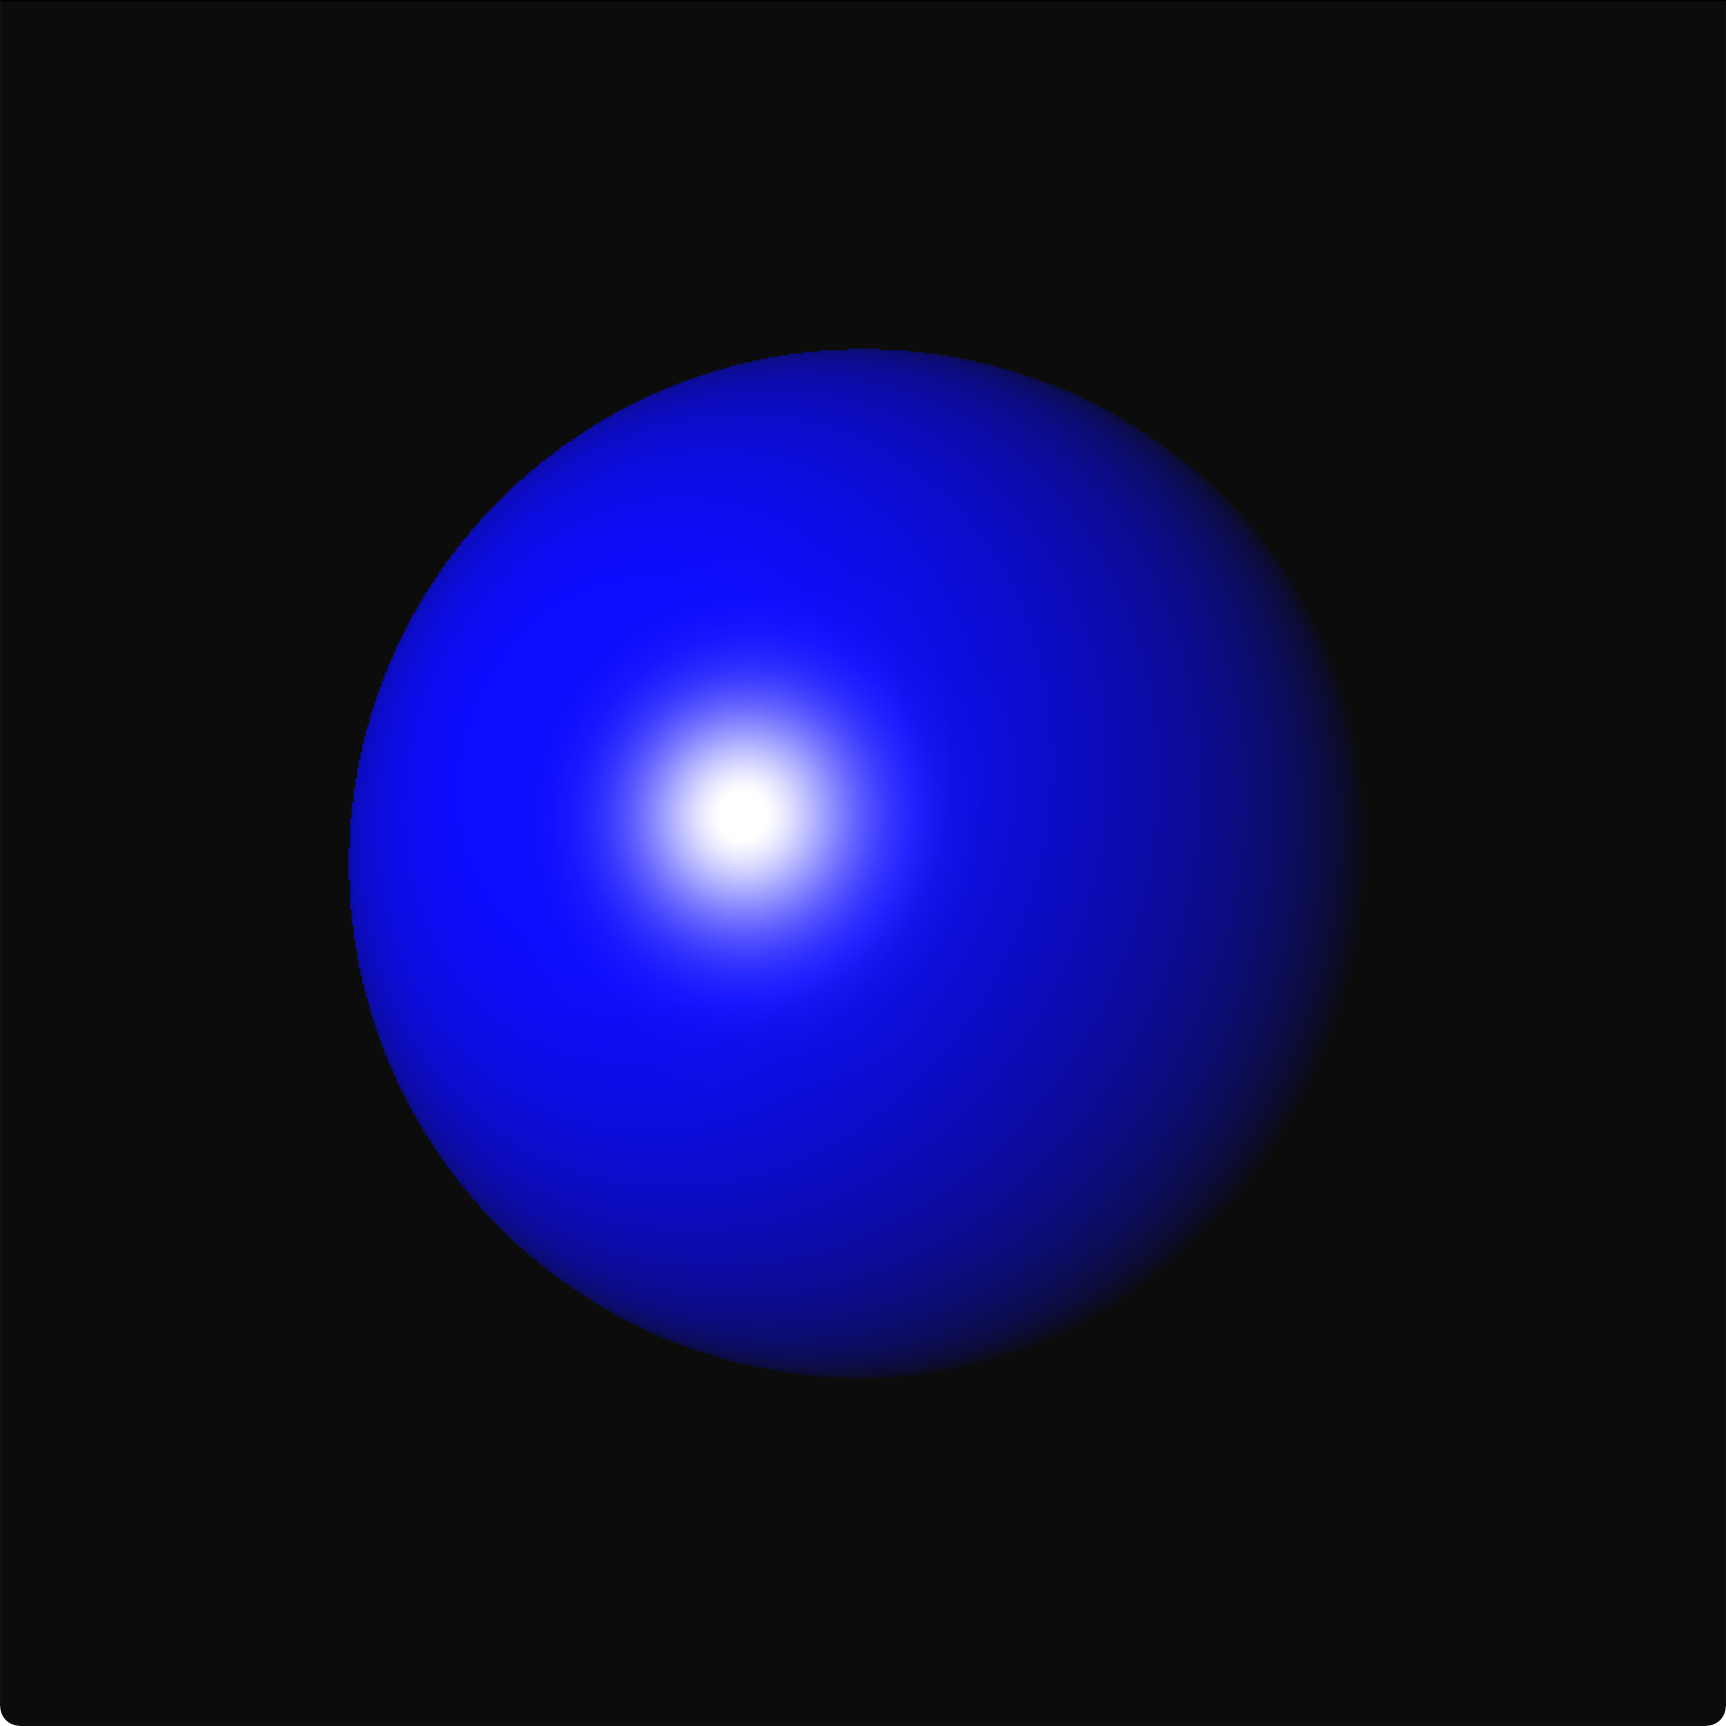
\includegraphics[width=8cm]{render}
\centering
\caption{Image rendered by the raytracer - single sphere in a blue color with light higlight on it}
\end{figure}

\begin{table}[ht]
\centering
\caption{Run-times of the GPU ray tracing algorithm depending on the block size (1000x1000 pixel) after three measurements}
\begin{tabular}{|r|r|r|r|r|}
Block size & Measurement 1 & Measurement 2 & Measurement 3 & Average \\
\hline
2 & 1.619552s & 1.617910675s & 1.877738284s & 1.705066986s \\
4 & 1.694843s & 1.771215823s & 1.74922937s & 1.738429398s \\
8 & 1.798312s & 1.840904832s & 1.765917719s & 1.801711517s \\
16 & 1.810418s & 1.876185735s & 1.961402516s & 1.88266875s \\
32 & 1.644953s & 1.918981885s & 1.923872876s & 1.829269253s \\
64 & 1.601591s & 1.54319824s & 1.692520928s & 1.612436723s \\
128 & 1.58987s & 1.550428561s & 1.575339408s & 1.571879323s \\
256 & 1.620525s & 1.54205651s & 1.719747472s & 1.627442994s \\
\end{tabular}
\end{table}

\begin{table}[ht]
\centering
\caption{Run-times (in s) of the GPU ray tracing algorithm depending on the image resolution (with block size of 128)}
\begin{tabular}{|r|r|r|r|r|r|r|}
100x100 & 200x200 & 500x500 & 1000x1000 & 2000x2000 & 5000x5000 & 10000x10000 \\
\hline
0.023476 & 0.088649 & 0.445735 & 1.7008 & 6.021729 & 37.37126 & 150.599173 \\
0.020846 & 0.073339 & 0.383999 & 1.502596 & 5.926812 & 37.36544 & 151.34943 \\
0.022106 & 0.078558 & 0.356222 & 1.50109 & 5.968768 & 37.739508 & 150.887118 \\
0.018674 & 0.074268 & 0.369011 & 1.490234 & 6.000431 & 37.675598 & 151.005461 \\
0.0164 & 0.067305 & 0.373659 & 1.478384 & 6.01874 & 37.776637 & 151.139262 \\
0.016731 & 0.06745 & 0.379556 & 1.490041 & 5.998759 & 37.660936 & 151.170938 \\
0.016029 & 0.063579 & 0.372769 & 1.483943 & 5.953615 & 37.723215 & 150.675566 \\
0.016651 & 0.060664 & 0.380712 & 1.517852 & 5.960818 & 37.714795 & 151.164509 \\
0.017792 & 0.050732 & 0.381688 & 1.496121 & 5.992531 & 37.690435 & 150.848411 \\
0.016156 & 0.054281 & 0.367019 & 1.495951 & 5.978727 & 37.602042 & 151.120895 \\
\end{tabular}
\end{table}

\begin{table}[ht]
\centering
\caption{Summary of the GPU algorithm measurements}
\begin{tabular}{|r|r|r|r|r|r|r|r|}
Resolution n (nXn)& 100 & 200 & 500 & 1000 & 2000 & 5000 & 10000 \\
\hline
Average time (in s) & 0.018 & 0.068 & 0.381 & 1.516 & 5.982 & 37.632 & 150.996 \\
Standard deviation & 0.00 & 0.01 & 0.02 & 0.07 & 0.03 & 0.15 & 0.24 \\
Seconds per pixel & 1.85e-06 & 1.70e-06 & 1.52e-06 & 1.52e-06 & 1.50e-06 & 1.51e-06 & 1.51e-06 \\
\end{tabular}
\end{table}

\begin{table}[ht]
\centering
\caption{Run-times (in s) of the CPU ray tracing algorithm depending on the image resolution}
\begin{tabular}{|r|r|r|r|r|r|r|}
100x100 & 200x200 & 500x500 & 1000x1000 & 2000x2000 & 5000x5000 & 10000x10000 \\
\hline
0.015669 & 0.063638 & 0.397402 & 1.513684 & 5.841313 & 35.976081 & 142.956475 \\
0.017002 & 0.058923 & 0.36504 & 1.549204 & 5.766883 & 35.723961 & 153.411116 \\
0.015566 & 0.055952 & 0.361869 & 1.424477 & 5.6201 & 35.152361 & 150.568681 \\
0.01451 & 0.055964 & 0.388553 & 1.498511 & 5.74655 & 35.566392 & 150.627749 \\
0.014419 & 0.056776 & 0.376333 & 1.43709 & 5.644908 & 35.34829 & 144.039645 \\
0.014223 & 0.057432 & 0.38793 & 1.468248 & 5.787562 & 35.537739 & 142.894829 \\
0.014224 & 0.064642 & 0.407985 & 1.433794 & 5.664931 & 35.449437 & 149.078384 \\
0.014057 & 0.058934 & 0.372597 & 1.4172 & 6.44838 & 35.217112 & 145.973658 \\
0.014245 & 0.058767 & 0.383913 & 1.473291 & 5.921579 & 35.226802 & 142.473777 \\
0.014296 & 0.058913 & 0.380276 & 1.433051 & 5.799808 & 35.259792 & 142.440786 \\
\end{tabular}
\end{table}

\begin{table}[ht]
\centering
\caption{Summary of the CPU algorithm measurements}
\begin{tabular}{|r|r|r|r|r|r|r|r|}
Resolution n (nXn)& 100 & 200 & 500 & 1000 & 2000 & 5000 & 10000 \\
\hline
Average time (in s) & 0.015 & 0.059 & 0.382 & 1.465 & 5.824 & 35.446 & 146.447 \\
Standard deviation & 0.00 & 0.00 & 0.01 & 0.04 & 0.24 & 0.26 & 4.12 \\
Seconds per pixel & 1.48e-06 & 1.47e-06 & 1.53e-06 & 1.46e-06 & 1.46e-06 & 1.42e-06 & 1.46e-06 \\
\end{tabular}
\end{table}

\begin{figure}[ht] %\scriptsize
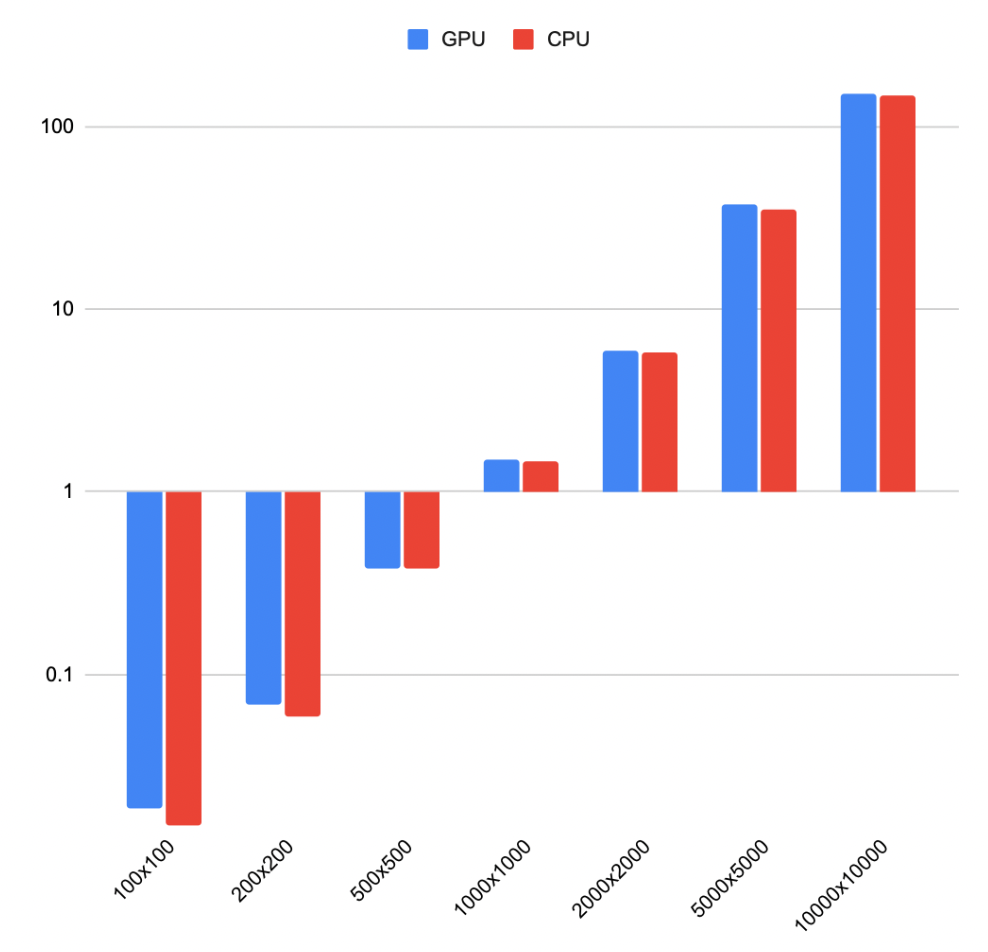
\includegraphics[width=8cm]{plot1}
\centering
\caption{GPU and CPU ray tracers render time in seconds (logarithmic scale - in seconds)}
\end{figure}

\begin{figure}[ht] %\scriptsize
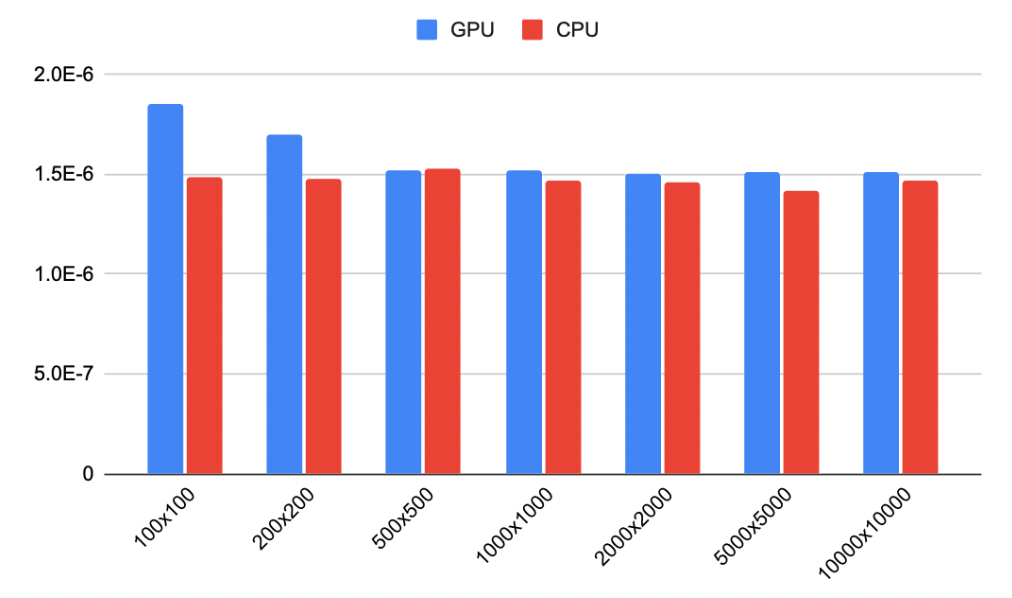
\includegraphics[width=8cm]{plot2}
\centering
\caption{Average time in seconds to render one pixel depending on the image resolution}
\end{figure}

\clearpage

\section{Discussion and conclusion}

While I expected the CPU version of the application to perform better with the low resolution renders because of the overhead which comes from copying the data back and forth to and from the GPU, it surprised me that it is also slightly faster when it comes to rendering images consisting of millions of pixels. I suspect two reasons behind the results. The first could be that this particular CPU is unproportionally more efficient than the GPU so that even though the parallelized GPU of the application is more efficient than the naive CPU one it’s still executing at a slightly faster pace. The second reason might be that the GPU implementation, even though it’s parallelized, it’s not efficient enough to overcome memory transfer time overhead. The thing to keep in mind with these results is that the rendered scene is very simple and the results could change if the scene would consist of multiple elements and not only one sphere, and then the GPU version should benefit more from the parallelization than currently. Another observation I made is that time of execution is highly correlated with the number of rendered pixels as it can be clearly deducted when we look at the average time required to render one pixel which stays stable regardless of the image resolution (around $1.51e-06$s/pixel with the GPU version and $ 1.46e-06 $s/pixel with the CPU version). What also can be observed is that for the GPU ray tracer is the fact that the time to generate pixels decreases until it plateaus after the 500x500 pixels render which would suggest that the data transfer time overhead becomes less relevant with the increase of the image resolution. Regardless of the reason behind that, the conclusion is that for particular implementations and scenes the CPU implementation could be slightly faster than the GPU one.


\singlespacing
\vspace{1cm}
\printbibliography
\end{document}
